\chapter{PENDAHULUAN}
\label{chap:pendahuluan}

% Ubah bagian-bagian berikut dengan isi dari pendahuluan

Penelitian ini di latar belakangi oleh berbagai kondisi yang menjadi acuan. Selain itu juga terdapat beberapa permasalahan yang akan dijawab sebagai luaran dari penelitian.

\section{Latar Belakang}
\label{sec:latarbelakang}

Menjaga kebersihan merupakan salah satu kunci untuk menjaga kesehatan tubuh, tubuh yang bersih dapat menghindarkan kita dari berbagai penyakit terutama yang berasal dari lingkungan disekitar kita. Kita sering kali menyentuh benda - benda di sekitar seperti gadget, komputer, gagang pintu, meja, lemari, dan lain sebagainya. Akan tetapi, banyak yang tidak sadar bahwa benda benda tersebut seringkali menjadi sarang bagi bakteri \& virus yang dapat menyebabkan penyakit. 

Ketika menyentuh benda benda tersebut, kuman – kuman yang ada akan berpindah dan menyebar di tangan kita, kemudian ketika kita menyentuh orang lain, maka kuman penyebab penyakit itu akan berpindah dan menyebar ke tubuh orang tersebut. Pada akhirnya Ketika kita menyentuh bagian – bagian di tubuh seperti mata, hidung dan mulut, maka kuman tersebut akan masuk ke tubuh kita dan menyebabkan penyakit. Oleh karena itu mencuci tangan merupakan hal yang paling utama dalam menjaga kesehatan tubuh dan mencegah penyebaran penyakit.

Pada saat penelitian ini berlangsung, 2020 - 2021, sedang marak terjadinya pandemi virus SARS-CoV-2 (Severe Acute Respiratory Syndrome – Corona Virus – 2) atau yang biasa disebut COVID-19 (Corona Virus Desease – 2019)\cite{cit:copid}. Bahkan pada hari ini, 8 Juni 2021, tercatat 174,429,426 kasus COVID-19 di dunia dan 3,753,525 diantaranya meninggal dunia \cite{cit:covidcase}

\newpage
\begin{figure}[ht]
	\centering
	
	% Ubah dengan nama file gambar dan ukuran yang akan digunakan
	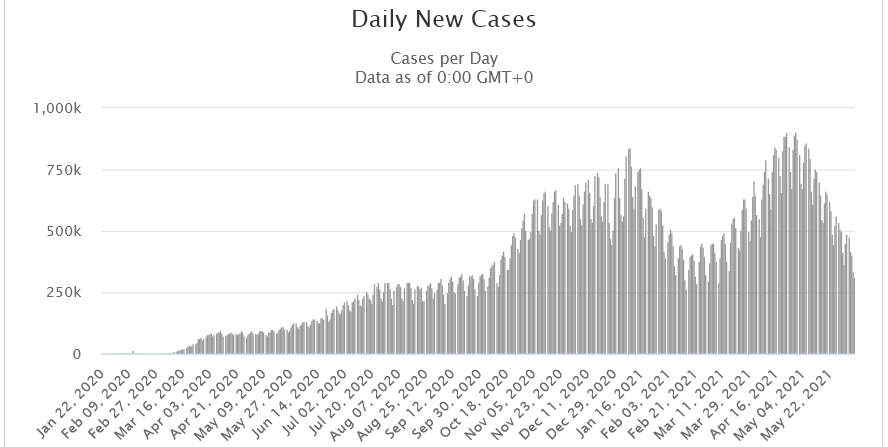
\includegraphics[width=0.9\columnwidth]{gambar/worldometer.PNG}
	
	% Ubah dengan keterangan gambar yang diinginkan
	\caption{Grafik Perkembangan Kasus \emph{COVID-19} \citep{cit:covidcase}.}
	\label{fig:covidstat}
\end{figure}

Virus ini menyerang sistem pernafasan yang menyebabkan pengidapnya kesulitan bernafas, kekurangan oksigen, hingga kematian. Virus ini sangat mudah untuk menyebar terutama melalui \emph{droplets} (percikan air) yang terjadi ketika bersin, batuk, dan bicara sekalipun. Droplets ini akan menempel ke benda - benda dan tubuh kita. Hanya dengan menyentuh benda atau bagian tubuh yang terkontaminasi kemudian tanpa sadar menyentuh mata, hidung ataupun mulut, maka virus tersebut akan masuk ke tubuh dan merusak sel paru-paru yang akhirnya menyebabkan gangguan pernafasan bahkan kematian.

Walaupun kebiasaan cuci tangan meningkat selama pandemi COVID-19 \cite{cit:cucisabun} banyak orang yang masih asal – asalan ketika mencuci tangan lantaran terburu-buru maupun hal lainnya. Menurut hallosehat.com \cite{cit:salahcuci} , masih banyak kesalahan dalam mencuci tangan yang sering dilakuk-an oleh masyarakat, diantaranya waktu mencuci tangan yang terlalu cepat dan kebiasaan masyarakat yang hanya menggosok talapak tangan saja ketika sedang mencuci tangan. Akan tetapi tidak memung-kinkan untuk dilakukannya pemantauan 7x24 jam oleh manusia terhadap pengunjung di tempat umum seperti mall dan tempat wisata lainnya demi memastikan pengunjung telah mencuci tangan dengan be-nar, terutama di masa pandemi COVID-19 ini yang mana masyarakat dihimbau untuk menjaga jarak untuk mencegah penularan.

\section{Permasalahan}
\label{sec:permasalahan}

Dari permasalahan tersebut maka permasalahan yang di ambil dalam penelitian tugas akhir ini adalah menemukan cara mendeteksi apakah seseorang sudah mencuci tangan dengan baik. Untuk itu diperlukan sebuah sistem klasifikasi gerakan mencuci tangan yang kemudian dapat dikembangkan lagi untuk menilai apakah orang tersebut telah mencuci tangannya dengan baik dan benar tanpa perlu dilakukannya pemantauan langsung oleh manusia

\section{Tujuan}
\label{sec:Tujuan}

Tujuan dari tugas akhir ini adalah membuat sebuah sistem yang dapat mengklasifikasikan gerakan mencuci tangan

\section{Batasan Masalah}
\label{sec:batasanmasalah}

Untuk memfokuskan permasalahan yang diangkat maka dilakukan pembatasan masalah. Batasan-batasan masalah tersebut di antaranya adalah:

\begin{enumerate}[nolistsep]
	
  \item Sistem Hanya berfokus pada Klasifikasi Gerakan Mencuci Tangan
  
  \item Metode Klasifikasi yang digunakan adalah metode \emph{Image Classification} berbasis CNN dengan mengaplikasikan Moving Average pada hasil prediksinya 
  
  \item \emph{Base Model} dalam Klasifikasi ini menggunakan \emph{EfficientNet}\cite{cit:effnet} dengan \emph{Weight Checkpoint} \emph{NoisyStudent}\cite{cit:noisy}
  
  \item Dataset yang digunakan berasal dari Kaggle Hand Wash Dataset Sample dan Dataset Pribadi

  \item Metode pengambilan data pribadi adalah menggunakan satu kamera dengan posisi dan sudut yang tetap
  
  \item Dikarenakan Kondisi Pandemi COVID-19 \cite{cit:copid}, Penelitian hanya akan dilakukan di sekitar tempat tinggal penulis dengan menerapkan \emph{Physical Distancing} demi mencegah terjadinya penyebaran penyakit
  
\end{enumerate}

\newpage
\section{Sistematika Penulisan}
\label{sec:sistematikapenulisan}

Laporan penelitian tugas akhir ini tersusun dalam sistematika dan terstruktur sehingga mudah dipahami dan dipelajari oleh pembaca maupun seseorang yang ingin melanjutkan penelitian ini. Alur sistematika penulisan laporan penelitian ini yaitu:

\begin{enumerate}[nolistsep]

  \item \textbf{BAB I Pendahuluan}

  Bab ini berisi uraian tentang latar belakang permasalahan, penegasan dan alasan pemilihan judul, sistematika laporan, tujuan, dan metodologi penelitian.
  
  \vspace{2ex}

  \item \textbf{BAB II Tinjauan Pustaka}

  Bab ini berisi tentang uraian secara sistematis teori-teori yang berhubungan dengan permasalahan yang dibahas pada penelitian ini. Teori-teori ini digunakan sebagai dasar dalam penelitian, yaitu informasi terkait Deep Learning, Convolutional Neural Network (CNN), EfficientNet dan teori-teori penunjang lainya.

  \vspace{2ex}

  \item \textbf{BAB III Desain dan Implementasi Sistem}

  Bab ini berisi tentang penjelasan-penjelasan terkait eksperimen yang akan dilakukan, langkah-langkah pengambilan data video dan proses klasifikasi gerakan mencuci tangan, serta analisis performa dari sistem. Guna mendukung itu digunakanlah blok diagram atau workflow agar sistem yang akan dibuat dapat terlihat dan mudah dibaca untuk implementasi pada pelaksanaan tugas akhir.

  \vspace{2ex}

  \item \textbf{BAB IV Pengujian dan Analisa}

  Bab ini menjelaskan tentang hasil serta analisis yang dida-patkan dari pengujian yang dilakukan mulai dari hasil pengujian \emph{model evaluation}, \textit{Confusion Matrix}, \textit{precission}, \textit{f1-score}, Pengujian pada video cuci tangan serta rekomendasi penerapan sistem.

  \vspace{2ex}

  \item \textbf{BAB V Penutup}

  Bab ini merupakan penutup yang berisi kesimpulan yang di-ambil dari penelitian dan pengujian yang telah dilakukan. Sar-an dan kritik yang membangun untuk pengembangan lebih lanjut juga dituliskan pada bab ini.

\end{enumerate}
